\documentclass[11pt,a4paper]{article}
\usepackage[margin=2.4cm]{geometry}
\usepackage{graphicx}
\usepackage{caption}
\usepackage{amsmath}
\usepackage{amssymb}
\usepackage{xcolor}
\usepackage[colorlinks=true,linkcolor=blue!50!black,urlcolor=blue!50!black,citecolor=blue!50!black]{hyperref}
\graphicspath{{figs/}}

\newcommand{\He}[1]{$^{#1}$He}
\newcommand{\sM}{\sigma_{\mathrm{M1}}}
\newcommand{\sE}{\sigma_{\mathrm{E0}}}
\newcommand{\sng}{\sigma_{n\gamma}}
\newcommand{\snp}{\sigma_{np}}
\newcommand{\aipc}{\alpha_{\mathrm{IPC}}}

\title{\vspace{-1.2cm}
  {\Large\bfseries \He{3}$(n,\cdot)$\He{4} capture cross sections and the IPC
   pair yield}\\[2mm]
  {\large The measured M1$+$E1 radiative capture, the $\gamma$-dark E0, and the
   $e^+e^-$ yield that follows from $\sigma\times$(pair fraction)}}
\author{Dylan Neff}
\date{15 June 2026 \\[2mm]
  {\small\itshape Internal note --- informal. Drafted by Claude (Anthropic AI
  assistant) under D.~Neff's direction; \\ physics, numbers and text
  reviewed by D.~Neff.}}

\begin{document}
\maketitle
\vspace{-0.8cm}

%=============================================================================
\section*{Part 0 --- Summary}

\noindent\textbf{In plain words.} The E0 transition is interesting but it does
\emph{not} rescue the thermal measurement. As the neutron energy drops, the
$\gamma$-dark E0 mode does turn on --- but its capture cross section is still
expected to be $\sim$100--1000$\times$ smaller than the M1
($\sE=f\,\sM$, $f\sim10^{-2}$--$10^{-3}$). That deficit is offset because E0 is
$\gamma$-forbidden, so \emph{every} E0 capture makes an $e^+e^-$ pair, whereas
only $\sim3.5\times10^{-3}$ of M1 photons internally convert --- E0 \emph{skips}
that penalty (a $\sim$300$\times$ relative boost). The two $\sim10^{-3}$ factors
roughly cancel, leaving E0 pair (hence X17) production \emph{the same order as}
the M1 in the sub-keV: at best a factor of $\sim$2--3 on the thermal statistics,
\textbf{not nearly enough to save that measurement}. At high $E_n$ the E0 adds
essentially nothing, since the M1$+$E1 (E1/giant-dipole) dominates and the E0 has
died away. \emph{This is outside the author's expertise and pushes the current
limit of what AI can do; the calculations were cross-checked but the note should
be read skeptically --- insights and holes welcome.}

\medskip

\begin{center}
\fcolorbox{blue!40!black}{blue!4}{%
\begin{minipage}{0.95\textwidth}
\vspace{3pt}
The capture cross section factorises as
$\sigma = \sigma_{\rm form}\times(\Gamma_X/\Gamma_{\rm tot})$ --- \textbf{form the
\He{4}$^*$ state, then radiate to the ground state rather than break up.} Two
consequences drive this note:
\begin{itemize}\setlength\itemsep{1pt}
  \item \textbf{The photon-emitting capture (M1$+$E1) is MEASURED} --- it is the
    ENDF \He{3}$(n,\gamma)$\He{4} cross section (55\,\textmu b at thermal, the
    classic value), with the M1-dominated $1/v$ at low $E_n$ and the E1/GDR rise
    toward MeV. \textbf{Only the $\gamma$-dark E0 is estimated:}
    $\sE = f\,\sM$, $f\sim10^{-3}$--$10^{-2}$, sitting 2--3 decades below at
    thermal (and further below toward MeV, as the E1 rises and the E0 dies).
  \item \textbf{The IPC ($e^+e^-$) yield is just $\sigma\times$(pair fraction):}
    $\times\aipc\approx3.5\times10^{-3}$ for M1$+$E1 (only the internal-pair tail
    of the photon makes a pair), $\times1$ for E0 ($\gamma$-dark $\Rightarrow$
    100\,\% pairs). Multiplying the measured curve \emph{down} by $\aipc$ while
    leaving E0 alone lifts E0 by $1/\aipc\approx285$: \textbf{the two pair yields
    become COMPARABLE at thermal/sub-keV} (E0/M1E1 $=f/\aipc\approx0.3$--3),
    while M1$+$E1 wins at MeV.
  \item \textbf{The dominant uncertainty is $f$} ($\sim$1 decade); the measured
    $\sng$ is firm and $\aipc$ contributes only $\sim\times1.8$.
\end{itemize}
\vspace{3pt}
\end{minipage}}
\end{center}

%=============================================================================
\section{The cross section is a product: form $\times$ radiate}

For capture through a compound \He{4}$^*$ state of spin $J$,
\[
\sigma(n,X)\;=\;\underbrace{\frac{\pi}{k^2}\,g_J\,\frac{\Gamma_n(E)\,
  \Gamma_{\rm tot}}{(E-E_r)^2+(\Gamma_{\rm tot}/2)^2}}_{\sigma_{\rm form}\ \ \text{(form the state)}}
\;\times\;\underbrace{\frac{\Gamma_X}{\Gamma_{\rm tot}}}_{\text{(radiate as }X\text{)}}.
\]
The total width is almost all \textbf{breakup} ($\Gamma_{\rm tot}\approx\Gamma_n
+\Gamma_p$, the (n,p)t channel), so the radiative branch is a $\sim10^{-8}$
sliver --- that is why capture is rare. Per channel,
$\sM=\sigma_{\rm form}(1^+)\,\Gamma_{\rm M1}/\Gamma_{\rm tot}$ and
$\sE=\sigma_{\rm form}(0^+)\,\Gamma_{\rm E0}/\Gamma_{\rm tot}$, so
\[
f\equiv\frac{\sE}{\sM}=\underbrace{\frac{\sigma_{\rm form}(0^+)}
  {\sigma_{\rm form}(1^+)}}_{\sim1\text{--}2\ (\text{rough})}\times
  \underbrace{\frac{\Gamma_{\rm E0}}{\Gamma_{\rm M1}}}_{\text{the unknown}}.
\]
(\He{4} capture is mostly \emph{direct}, so ``form then decay'' is not a literal
two-step process --- but the cross section still separates into a
kinematic/penetrability factor $\times$ an EM-strength factor, which is what
matters here. The formation side is detailed in
\texttt{docs/e0\_branch/doorway\_states\_note.md}.)

\subsection{Which \He{4}$^*$ state forms (the formation factor)}

The states available near the $n+{}$\He{3} threshold (20.58\,MeV) are the broad,
overlapping \He{4} levels of the TUNL $A=4$ evaluation \cite{tunl}
(Fig.~\ref{fig:levels}). Two features set the formation:

\begin{center}
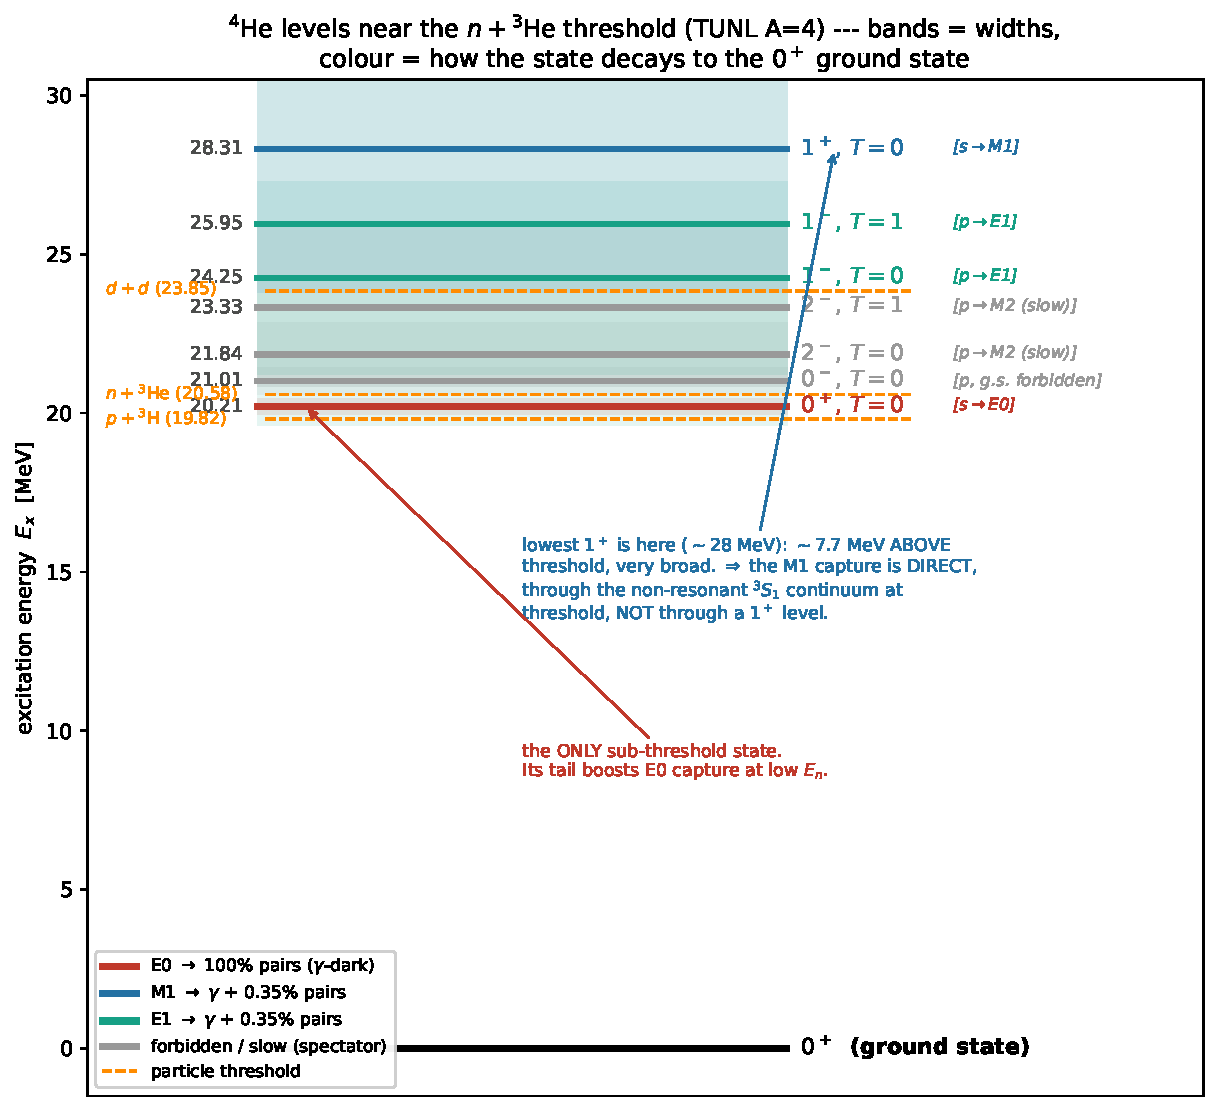
\includegraphics[width=0.80\textwidth]{fig_e0_levels.pdf}
\captionof{figure}{\He{4} levels near the $n+{}$\He{3} threshold (TUNL $A=4$).
  The levels are broad and overlapping, and the lowest $1^+$ sits $\sim$8\,MeV
  \emph{above} threshold --- there is no low-lying $1^+$.}
\label{fig:levels}
\end{center}

\begin{itemize}\setlength\itemsep{1pt}
  \item \textbf{The levels are broad} ($\Gamma\sim0.5$--13\,MeV, so
    $\Gamma\gtrsim|E_r|$): \He{4} has no sharp levels above threshold, so capture
    is \textbf{mostly direct/continuum} capture, modulated by broad structure
    rather than sharp resonant capture.
  \item \textbf{There is no low-lying $1^+$ level} (the lowest is $\sim$28\,MeV).
    So the M1 capture proceeds \emph{directly} through the continuum, while only
    the $0^+$ (a sub-threshold level at 20.21\,MeV, 0.37\,MeV below threshold) has
    a broad resonance assisting it.
\end{itemize}

\noindent Parity fixes the entrance orbital angular momentum, $\pi=(-1)^\ell$:
\begin{center}
\begin{tabular}{lll}
\hline
reached by & $\to$ states & energy behaviour \\
\hline
\textbf{s-wave} ($\ell=0$) & $0^+,\,1^+$ & no barrier --- rise as $1/v$, dominate at low $E_n$ \\
\textbf{p-wave} ($\ell=1$) & $0^-,\,2^-,\,1^-$ & barrier-suppressed --- switch on at sub-MeV/MeV \\
\hline
\end{tabular}
\end{center}

\noindent Two consequences feed the cross sections below: the $1^+$ (M1) is
\emph{pure direct} continuum capture --- giving the clean $1/v$, $55$\,\textmu b
\He{3}$(n,\gamma)$ with no thermal resonance --- while the $0^+$ (E0) is direct
\emph{plus} a sub-threshold boost ($\sim$10$\times$ at threshold relative to
1\,MeV), concentrating the E0 at the lowest $E_n$. The quantitative doorway
decomposition (and the correction of an earlier ``$1^+$ dominates'' artifact) is
in \texttt{docs/e0\_branch/doorway\_states\_note.md}.

\subsection{Which states can radiate to the ground state (the EM-strength factor)}

Whatever forms, \He{4}$^*$ almost always just breaks back up ($p+{}^3$H, the
(n,p)t reaction) and makes no pair; the rare EM drop to the $0^+$ ground state is
the only pair source, and \emph{what kind} of drop is fixed by $J^\pi$:

\begin{center}
\renewcommand{\arraystretch}{1.2}
\begin{tabular}{llcl}
\hline
State & $\to0^+$ g.s. & pairs? & role for our signal \\
\hline
\textbf{$0^+$} (20.21) & \textbf{E0} ($\gamma$ forbidden) & \textbf{100\,\%} & \textbf{E0 pair source} --- low $E_n$ \\
\textbf{$1^+$} ($^3S_1$) & M1 & 0.35\,\% & \textbf{M1 pair source} --- the ordinary 55\,\textmu b \\
\textbf{$1^-$} (24--26) & E1 & 0.35\,\% & \textbf{E1 pair source} --- rises toward MeV \\
$0^-$ (21.01) & forbidden & --- & spectator (breaks up) \\
$2^-$ (21.84) & M2 (too slow) & $\sim$0 & spectator \\
\hline
\end{tabular}
\end{center}

\noindent The decisive line is $0^+\!\to0^+$: a real photon is forbidden
($0\to0$ kills every photon multipole, M1 included), so the \emph{only} outlet is
an $e^+e^-$ pair --- \textbf{100\,\% pairs, $\gamma$-dark}, invisible to
ENDF/Geant4. The $1^+$ and $1^-$ emit a 20.6\,MeV $\gamma$ with the small
internal-pair tail $\aipc$ (so M1 is a \emph{different} capture channel from E0,
not its photon partner). The $0^-$ ($0\to0$ plus parity flip forbids even E0) and
$2^-$ (M2 far too slow at 20\,MeV) are spectators. This is why the EM-strength
factor reduces to the three source states $\{0^+,1^+,1^-\}$ used throughout.

%=============================================================================
\section{The capture cross sections: measured vs estimated}

\begin{center}
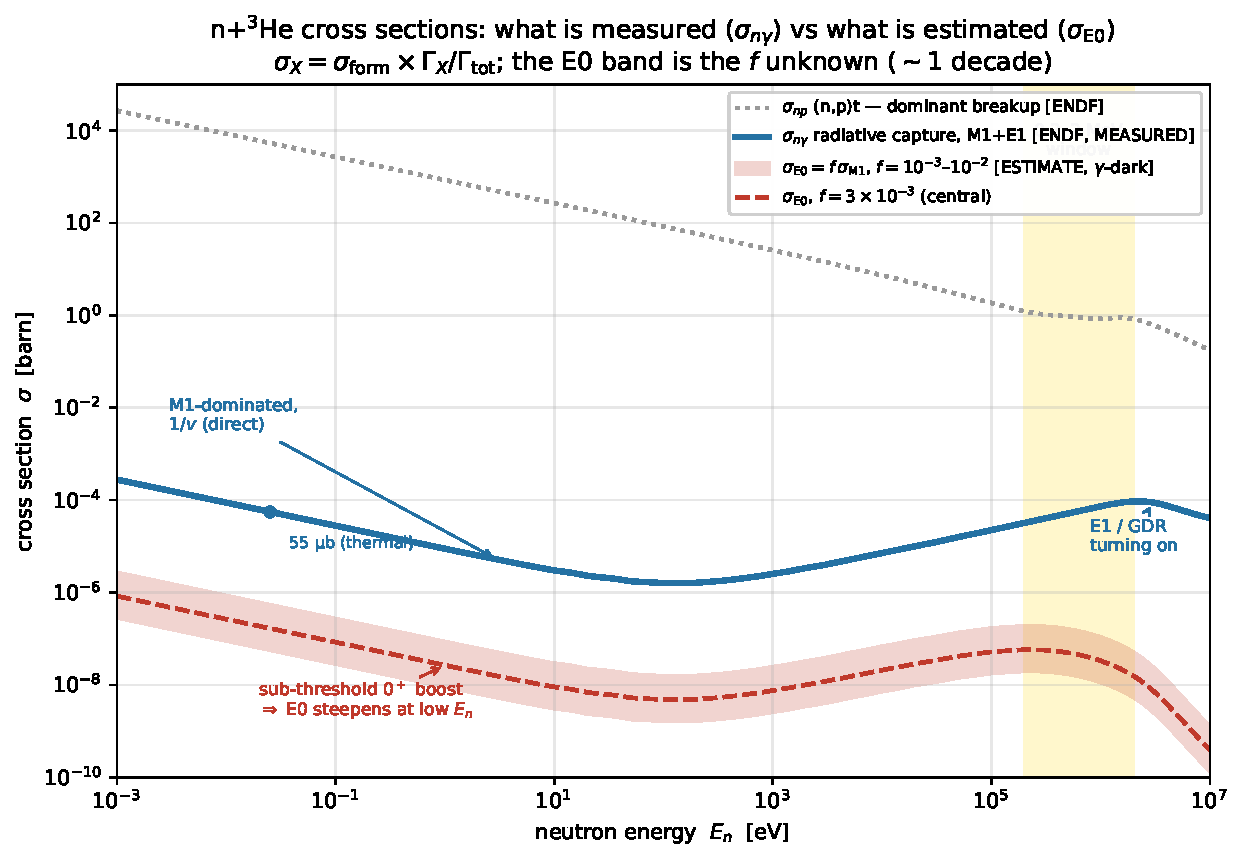
\includegraphics[width=0.92\textwidth]{fig_e0_xsec.pdf}
\end{center}

\noindent Reading the figure:
\begin{itemize}\setlength\itemsep{1pt}
  \item \textbf{$\snp$ (grey, dotted)} --- the dominant (n,p)t breakup, 5330\,b
    at thermal. This \emph{is} $\Gamma_{\rm tot}$, and the reference for ``rare.''
  \item \textbf{$\sng$ (blue, MEASURED)} --- total radiative capture (M1$+$E1),
    ENDF/B-VIII.0, 55\,\textmu b at thermal. The $1/v$ falloff is the
    M1-dominated direct capture; the rise toward MeV is the E1/giant-dipole
    strength (the $T=1$ $1^-$) turning on. \textbf{No estimation enters this
    curve.}
  \item \textbf{$\sE$ (red band, ESTIMATE)} --- the $\gamma$-dark E0 capture,
    $\sE=f\,\sM$ with the sub-threshold $0^+$ boost steepening it toward low
    $E_n$. The band is $f=10^{-3}$--$10^{-2}$; $\sE(\text{thermal})\approx
    0.055$--$0.55$\,\textmu b. Invisible to $\sng$ (it emits no photon).
\end{itemize}
The honest split is stark: a measured photon capture, and a $\gamma$-dark E0
capture 2--3 decades below it at thermal (further below toward MeV) whose
absolute height is the open $f$.

%=============================================================================
\section{The IPC pair yield: $\sigma\times$(pair fraction)}

The $e^+e^-$ yield is each cross section times its pair fraction --- $\times\aipc$
for the photon channel (only the internal-pair tail of the $\gamma$ becomes a
pair), $\times1$ for E0 (it makes nothing \emph{but} pairs):
\[
\sigma_{\rm pair}(\text{M1}+\text{E1})=\sng\times\aipc,\qquad
\sigma_{\rm pair}(\text{E0})=\sE\times1 .
\]
$\aipc\approx3.5\times10^{-3}$ at 20.6\,MeV (anchored to the measured
$^{12}$C 15.1\,MeV M1 IPC, $(3.3\pm0.5)\times10^{-3}$ \cite{ipc12c}, and the
high-energy IPC theory \cite{ss}; BrIcc's pair tables stop at 6\,MeV
\cite{bricc}; band $2.5$--$4.5\times10^{-3}$; Alberto's table uses
$2.1\times10^{-3}$).

\begin{center}
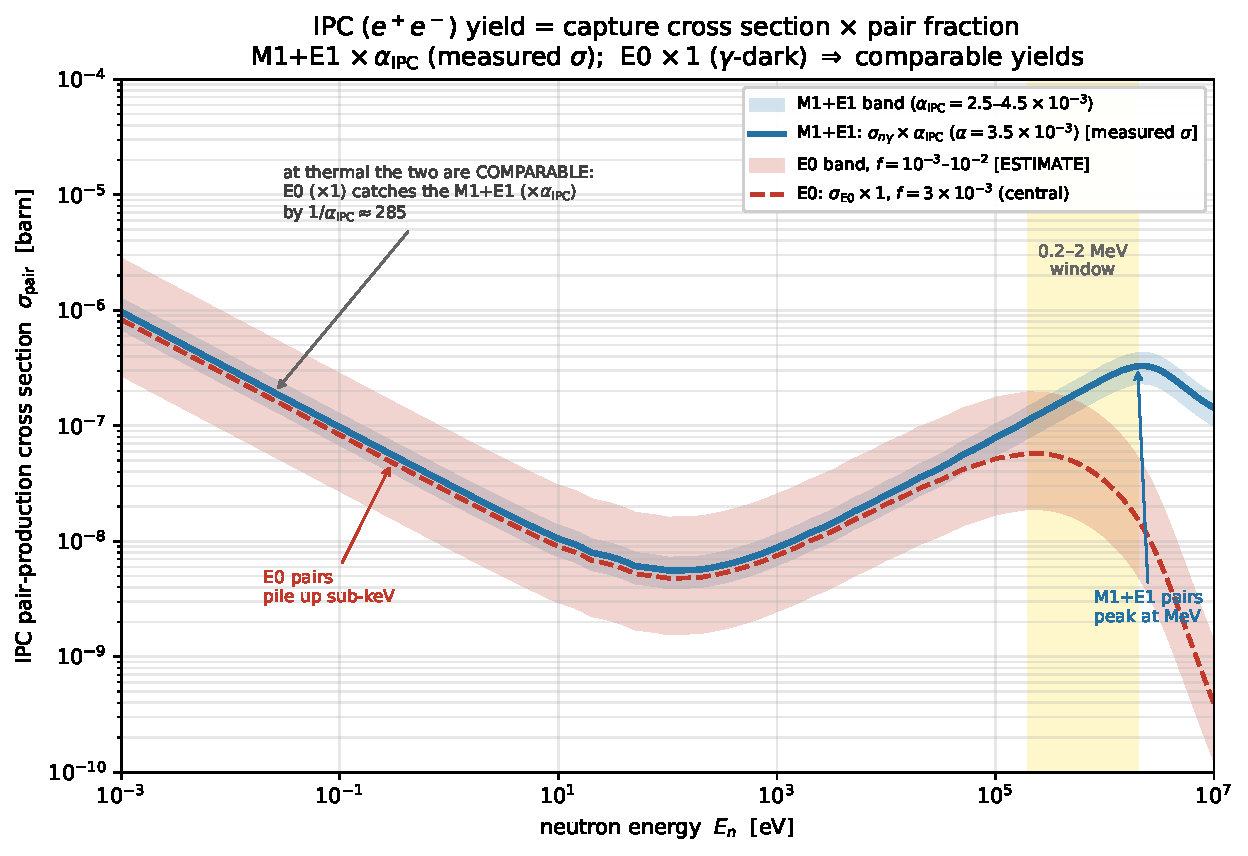
\includegraphics[width=0.92\textwidth]{fig_e0_ipcyield.pdf}
\end{center}

\noindent \textbf{The result.} Multiplying the measured curve \emph{down} by
$\aipc$ while leaving E0 \emph{unchanged} lifts E0 by $1/\aipc\approx285$
relative to M1$+$E1. The 4--5-decade gap of the capture figure \textbf{collapses}:
the two pair yields are \textbf{comparable at thermal} (at $E_n=25$\,meV,
$\sigma_{\rm pair}^{\rm M1+E1}=0.19$\,\textmu b vs $\sigma_{\rm pair}^{\rm E0}=
0.055$--$0.55$\,\textmu b, i.e. E0/M1E1 $=f/\aipc\approx0.3$--3). They then split
by energy --- \textbf{E0 pairs pile up sub-keV, M1$+$E1 pairs peak at MeV} --- so
the $\gamma$-dark channel matters precisely where the ordinary one is dead.

%=============================================================================
\section{X17 production, and the two scenarios}

X17 is produced as a sub-branch of the same transitions:
$\sigma_{\rm X17}=$ (IPC yield) $\times\,$BR$_{\rm X17}$ with
BR$_{\rm X17}=0.025$ (X17 per $e^+e^-$ pair, the project benchmark). Which
\emph{modes} contribute depends on the X17 quantum numbers, through one decisive
rule: a $0^+\!\to0^+$ (E0/monopole) transition can emit a massive boson only if
its $J^P$ allows $0^+\!\to0^++X$ ---

\begin{center}
\renewcommand{\arraystretch}{1.1}
\begin{tabular}{lcc}
\hline
X17 & $J^P$ & $0^+\!\to0^+$ emission \\
\hline
vector (dark photon) & $1^-$ & \textbf{allowed} ($L=1$) \\
scalar & $0^+$ & \textbf{allowed} ($L=0$) \\
pseudoscalar & $0^-$ & forbidden \\
axial-vector & $1^+$ & forbidden \\
\hline
\end{tabular}
\end{center}

\noindent The reason $0^+\!\to0^+$ is $\gamma$-dark is specifically that the
\emph{photon is massless} (transverse-only, cannot carry a monopole); X17 is
massive ($\sim$17\,MeV), so that argument does not apply --- \textbf{E0 is
$\gamma$-dark but not X17-dark}, and a vector/scalar X17 could even be relatively
\emph{enhanced} (it is not competing against the 0.35\,\% IPC tail of a real
$\gamma$, the same logic that makes E0 ``100\,\% pairs''). Two honest caveats
keep this from being a discovery: (i) the E0$\to$X17 branching is a
\emph{separate} unknown --- not the 2.5\,\% measured for the M1 line (different
multipole, phase space, coupling); we use 2.5\,\% only as a placeholder. (ii)
Whatever the branching, the rate is bounded by the (small) E0 \emph{capture}
rate, so X17-from-E0 stays $\lesssim$0.3/day produced (\S6, \S\ref{sec:stats}).

\noindent so the total X17 production splits into two scenarios, differing
\emph{only} by the $\gamma$-dark E0 channel:
\begin{itemize}\setlength\itemsep{1pt}
  \item \textbf{Scenario 1 (vector or scalar):} M1$+$E1 $+$ E0.
  \item \textbf{Scenario 2 (pseudoscalar or axial):} M1$+$E1 only.
\end{itemize}
(At the strict per-multipole level the M1/E1 couplings are also type-dependent;
we take ``X17 rides the measured M1$+$E1 strength'' as the working
approximation, so the clean scenario difference is the E0 piece.)

\begin{center}
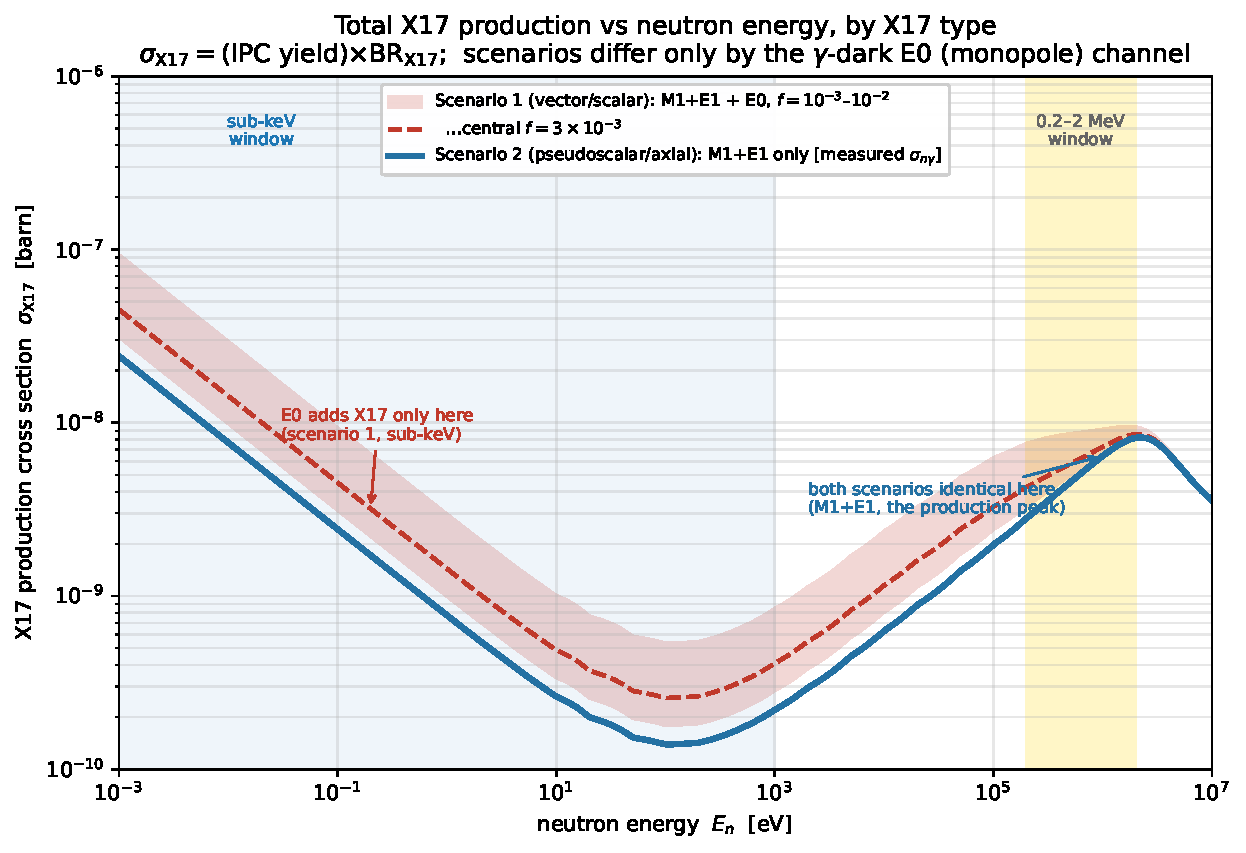
\includegraphics[width=0.92\textwidth]{fig_e0_x17.pdf}
\end{center}

\noindent The two scenarios are \textbf{identical at the MeV production peak}
(all M1$+$E1) and diverge only in the sub-keV region, where scenario~1 gets the
E0 band.

%=============================================================================
\section{From cross section to statistics}
\label{sec:stats}

To turn a cross section into a rate we fold in the simulated beam:
\[
\frac{N_X}{\text{day}}(E_n)=\underbrace{\phi(E_n)}_{\text{flux}}\times
  \underbrace{f_{\rm breakup}(E_n)}_{\substack{\text{fraction of beam}\\\text{interacting in gas}}}\times
  \underbrace{\frac{\sigma_X(E_n)}{\snp(E_n)}}_{\text{X per breakup}}\times
  \text{pulses/day},
\]
equivalently $N_X=N_{(n,p)}\times\sigma_X/\snp$ --- \textbf{the (n,p)t breakup,
counted directly in Geant4, is the luminosity monitor.} The clean part: even
where the gas is \emph{opaque} (sub-keV), the flux attenuation along the column
is set by the dominant (n,p) absorption, so it multiplies \emph{both} channels
by the same $(1-e^{-\tau_{np}})$ and \textbf{cancels in the ratio} ---
$N_X=N_{(n,p)}\,\sigma_X/\snp$ holds exactly. (For M1$+$E1 we instead use the
direct Geant4 $(n,\gamma)$ count, which bakes in flux/geometry/opacity already;
E0, absent from Geant4, is the one obtained via the ratio.)

\begin{center}
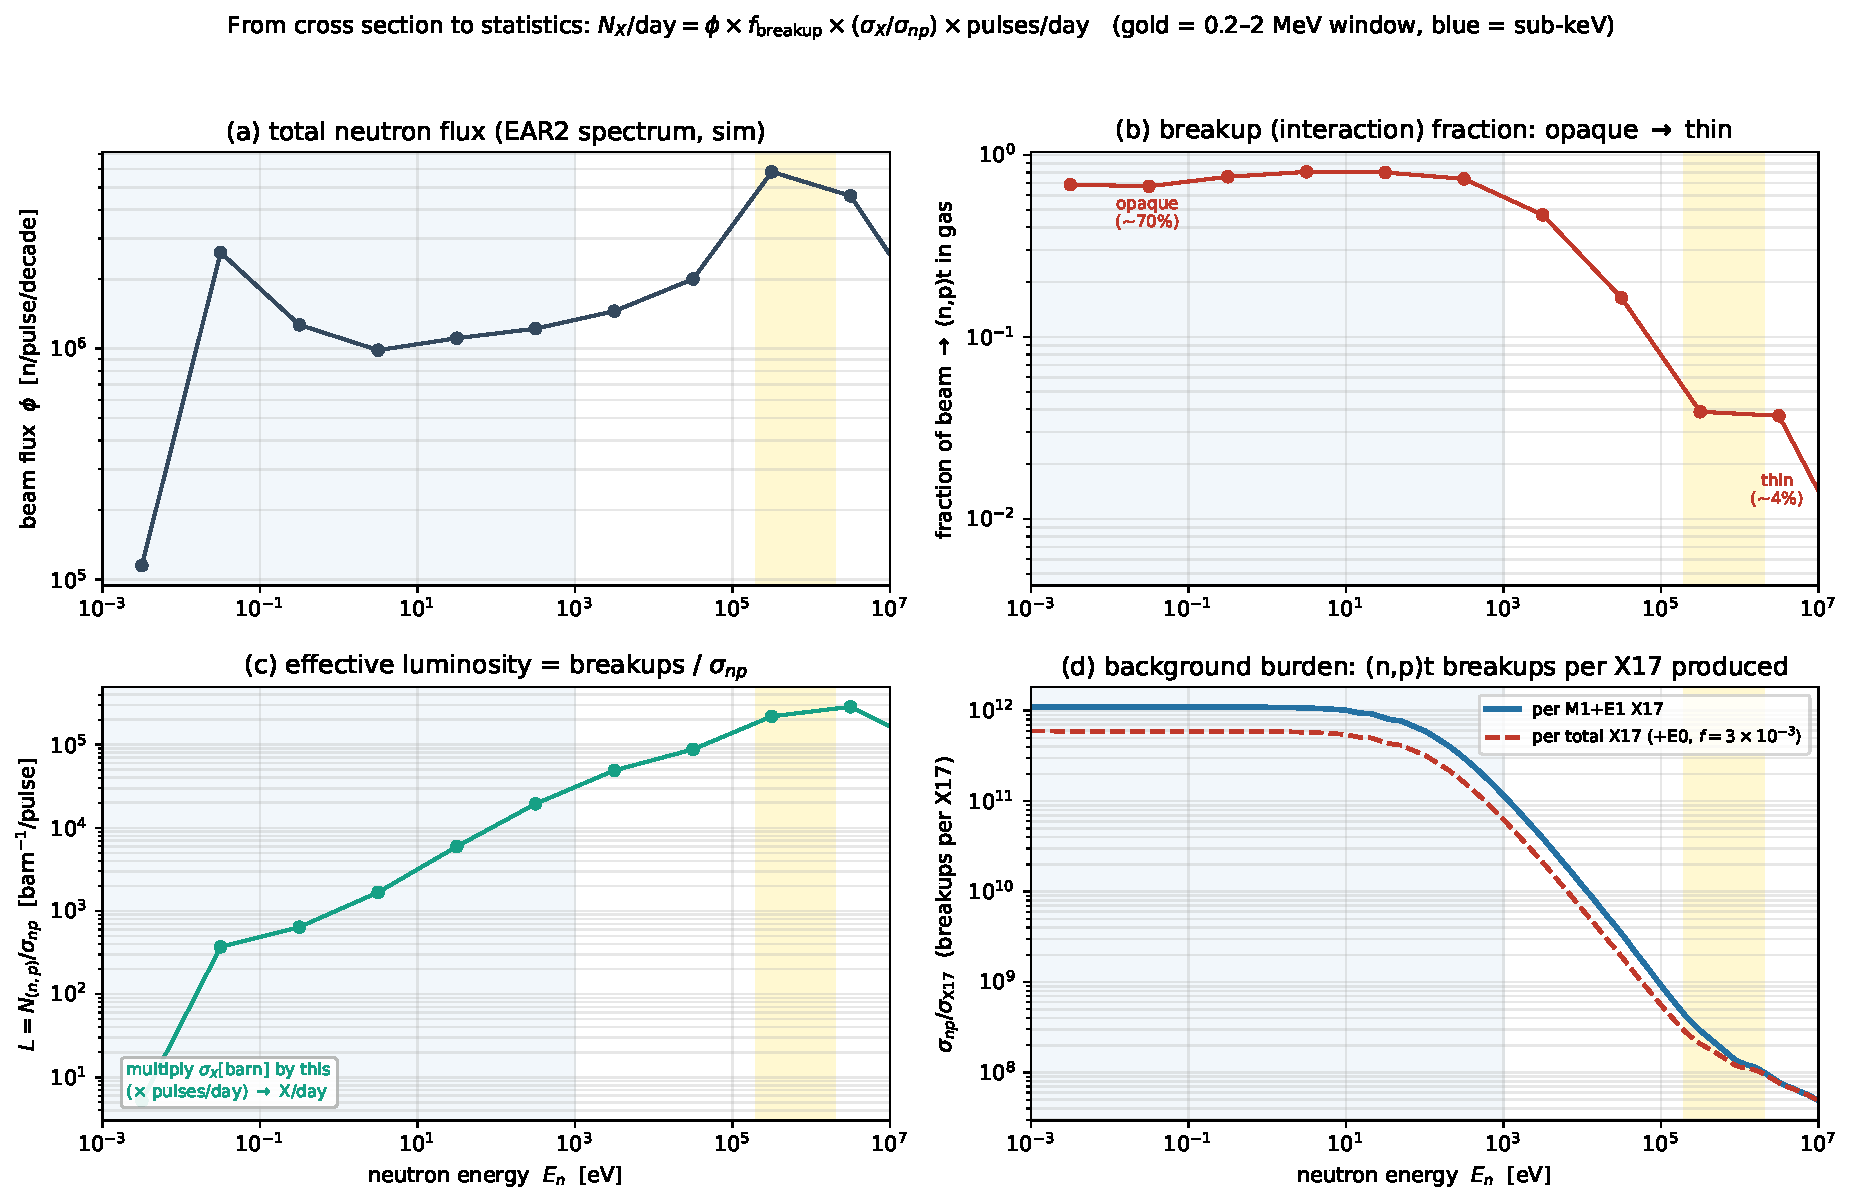
\includegraphics[width=0.98\textwidth]{fig_e0_lumi.pdf}
\end{center}

\noindent The four factors, vs energy: \textbf{(a)} the EAR2 flux $\phi$;
\textbf{(b)} the breakup fraction, $\sim$70\,\% (opaque) sub-keV falling to
$\sim$4\,\% (thin) at MeV; \textbf{(c)} the effective luminosity
$L=N_{(n,p)}/\snp$ --- multiply $\sigma_X$[barn] by this ($\times$pulses/day) to
get X/day; \textbf{(d)} the background burden, (n,p)t \emph{breakups per X17
produced}, which falls from $\sim$10$^{12}$ in the sub-keV to $\sim$10$^{8}$ at
MeV. Panel (d) is the quantitative reason the MeV window is favourable: $\sim$10$^4\times$
fewer breakups per signal than sub-keV. (The E0 channel, scenario~1, lowers the
burden at low $E_n$ --- red dashed --- but only into the $\sim$10$^{11}$ range.)

\subsection*{The daily statistics (the number we want)}

Folding the measured per-decade campaign flux (\texttt{mev\_rates.json}), the
\textbf{X17 produced per day} in the two windows:

\begin{center}
\renewcommand{\arraystretch}{1.25}
\begin{tabular}{lcc}
\hline
X17 produced / day & Scenario 2 & Scenario 1 (vector/scalar) \\
 & (M1$+$E1 only) & M1$+$E1 $+$ E0, $f=10^{-3}$–$10^{-2}$ \\
\hline
\textbf{high-energy window} (0.2--2\,MeV) & $37.4$ & $37.4$ (E0 adds $<0.004$) \\
\textbf{full sub-keV window} ($E_n<1$\,keV) & $0.15$ & $0.18$–$0.42$ \\
\hline
\end{tabular}
\end{center}

\noindent (Anchored $\aipc=3.5\times10^{-3}$; the high-energy row is
$22.5$/day with the table $\aipc=2.1\times10^{-3}$ --- the committed headline.
E0 \emph{alone} contributes $0.03$–$0.27$ X17/day in the sub-keV and
$<0.004$/day in the high-energy window.)

\textbf{What this says.} (i) The high-energy window carries the X17 rate ---
$\sim$22--37 produced/day --- and is \textbf{identical in both scenarios}: E0 is
irrelevant there, so the baseline measurement does not depend on the X17 type.
(ii) The sub-keV window is \textbf{starved either way}: even the most favourable
case (vector/scalar X17, $f=10^{-2}$) gives only $\sim$0.4 X17/day, $\sim$100$\times$
below the high-energy window; the E0 channel at best $\sim$2--3$\times$ the (tiny)
sub-keV M1$+$E1 rate. So a vector/scalar X17 would add a \emph{distinct sub-keV
signature}, but not significant \emph{statistics}.
(iii) These are \emph{produced}; recorded $\approx\times0.196$ (MM acceptance),
and the sub-keV window additionally requires a thermal trigger (the 0.2--2\,MeV
window is already in the 10\,\textmu s flash readout).

\subsection*{Everything folded: per day per decade}

\begin{center}

\includegraphics[width=\textwidth]{fig_e0_folded.pdf}
\end{center}

\noindent The full fold-down, per decade: X17 (left) and IPC pairs (right),
\emph{produced} and \emph{recorded} ($\times$ the MM-double geometric acceptance,
0.196 X17 / 0.236 IPC). Scenario~2 (blue) is M1$+$E1 only; scenario~1 (red band)
adds E0 over $f=10^{-3}$–$10^{-2}$. The MeV peak (gold window) carries the rate
and is scenario-independent; the sub-keV (blue) is where scenario~1's E0 lifts an
otherwise-dead region --- but to small absolute numbers. The boxed sums are the
window totals (produced $\to$ recorded). \emph{(Acceptance only; the sub-keV
recording additionally needs a thermal trigger, and these use at-rest acceptance
--- the $E_n$-boost correction is pending.)}

\subsection*{The trigger/readout window: what is actually recorded}

One more fold turns ``produced'' into ``recorded'': the detector only reads out
for a finite time after the proton pulse, and time-of-flight maps that window
onto neutron energy, TOF$(E_n)=L/v$ at $L=19.5$\,m. \textbf{This is what decides
whether E0 is ever seen.}
\begin{itemize}\setlength\itemsep{1pt}
  \item The \textbf{$\sim$10\,\textmu s flash readout} accepts only
    $E_n\gtrsim20$\,keV (TOF$=10$\,\textmu s $\Leftrightarrow$ 19.9\,keV). The
    0.2--2\,MeV window sits comfortably inside it.
  \item The \textbf{E0 pairs are sub-keV} (TOF $>45$\,\textmu s) --- they arrive
    \emph{after} the flash window closes. \textbf{Recorded E0 under the flash
    readout $\approx0$.} Only a dedicated \textbf{thermal trigger} recovers the
    sub-keV decades.
\end{itemize}

\noindent Folding acceptance ($\times0.196$ X17, $\times0.236$ IPC) and the two
readout schemes onto the windowed produced rates above
($\aipc=3.5\times10^{-3}$):

\begin{center}
\renewcommand{\arraystretch}{1.25}
\begin{tabular}{lccc}
\hline
recorded / day & produced & flash 10\,\textmu s & flash $+$ thermal \\
\hline
\multicolumn{4}{l}{\emph{X17 signal}}\\
\quad 0.2--2\,MeV (both scen.)      & $37.4$        & $7.3$ & $7.3$ \\
\quad sub-keV, scen.\,2 (M1$+$E1)   & $0.15$        & $0$   & $0.03$ \\
\quad sub-keV, scen.\,1 ($+$E0)     & $0.18$–$0.42$ & $0$   & $0.035$–$0.083$ \\
\hline
\multicolumn{4}{l}{\emph{IPC background pairs}}\\
\quad 0.2--2\,MeV                   & $1497$        & $353$ & $353$ \\
\quad sub-keV, no E0                & $6$           & $0$   & $1.4$ \\
\quad sub-keV, with E0              & $7$–$17$      & $0$   & $1.7$–$4$ \\
\hline
\end{tabular}
\end{center}

\noindent (With the table $\aipc=2.1\times10^{-3}$ the 0.2--2\,MeV rows scale by
$0.6$: X17 produced $22.5$, recorded $4.4$/day --- the committed headline. The
full-spectrum totals, integrating beyond 0.2--2\,MeV, are larger still:
$\sim$32.7 X17/day produced, $\sim$500 IPC pairs/day recorded under the flash
readout --- the MeV-note baseline.)

\textbf{What this means for the measurement.}
\begin{itemize}\setlength\itemsep{2pt}
  \item \textbf{The flash-readout run is unaffected by E0.} Its recorded rate is
    entirely M1/E1; E0 is sub-keV and arrives after the window, so leaving E0 out
    of the generator does not bias the baseline high-energy analysis.
  \item \textbf{A thermal trigger is the only way to reach E0}, and the prize is
    modest: $\lesssim$3 extra IPC pairs/day and $\lesssim$0.06 X17/day, sitting on
    the enormous sub-keV charged-particle load ($\sim$3$\times10^{5}$ (n,p)t per
    pulse in the opaque gas). The statistics exist in thermals, but the E0 pair
    signal is $f\times10^{-8}$ of them --- \textbf{S/B, not rate, is the obstacle.}
  \item \textbf{The generator action item is small and low-priority:} a third
    pair sub-generator at the $0^+$ transition energy with monopole kinematics,
    weighted by $N_{\rm E0}/N_{\rm M1/E1}$; it will not move the recorded spectra
    under the flash readout.
\end{itemize}

%=============================================================================
\section{Uncertainties}

\begin{center}
\renewcommand{\arraystretch}{1.2}
\begin{tabular}{lll}
\hline
piece & size of uncertainty & how to shrink \\
\hline
$\sng$ (M1$+$E1 capture) & small (evaluated data) & --- (measured) \\
$\aipc$ (pair fraction, M1$+$E1) & $\sim\times1.8$ (2.5--4.5$\times10^{-3}$) & high-energy IPC theory + $^{12}$C anchor \\
$\sigma_{\rm form}(0^+)/\sigma_{\rm form}(1^+)$ & $\sim\times2$--3 & \He{4} R-matrix reduced widths \\
\textbf{$f=\sE/\sM$} & \textbf{$\sim$1 decade ($10^{-3}$--$10^{-2}$)} & \textbf{\He{4} R-matrix $+$ $(e,e')$ monopole norm.} \\
\hline
\end{tabular}
\end{center}

\noindent \textbf{$f$ dominates by far}, so the E0 pair yield should be quoted as
an order-of-magnitude \emph{band}, not a central value (as drawn). The formation
ratio and $\aipc$ are sub-dominant and, for $f$, are already bundled into it.
A literature dig found the pieces but not the number: the \He{4} $0^+_2$ E0
strength \emph{is} measured (the MAMI monopole form factor \cite{kegel}, the
``$\alpha$-particle monopole puzzle'' \cite{puzzle}) and is a real, collective
transition --- but that is the \emph{decay-side} matrix element, and turning it
into a capture rate needs reaction theory; the ATOMKI \He{4} pair work
\cite{atomki} models its pairs as E1/M1 capture, not a clean E0 line; and no
calculation of \He{3}$(n,e^+e^-)$\He{4} exists. The bracket
$f\sim10^{-3}$--$10^{-2}$ is a transparent order-of-magnitude estimate
(statistical $^1S_0$ weight $\tfrac14$ as a floor, E0 having no real-photon mode
as a ceiling). The one calculation that turns the red band into a line is a
\He{4} multi-level R-matrix (Hale's evaluated system \cite{tunl}) for the
$^1S_0$ $n+{}$\He{3}$\to$g.s.\ E0 capture, normalised by the measured
\He{4}$(e,e')$ monopole strength.

%=============================================================================
\section*{Reproducing this note}
{\raggedright
Figures: \texttt{scripts/make\_e0\_cross\_section\_fig.py} (capture cross
sections, $\to$\texttt{fig\_e0\_xsec}),
\texttt{scripts/make\_e0\_ipc\_yield\_fig.py} (pair yield, $\to$
\texttt{fig\_e0\_ipcyield}), and
\texttt{scripts/make\_e0\_x17\_production\_fig.py} (X17 production $+$ the
window daily statistics, $\to$\texttt{fig\_e0\_x17}), and
\texttt{scripts/make\_e0\_luminosity\_fig.py} (the flux/breakup/luminosity
bridge, $\to$\texttt{fig\_e0\_lumi}), and
\texttt{scripts/make\_e0\_folded\_fig.py} (the folded per-day-per-decade result,
$\to$\texttt{fig\_e0\_folded}); all read \texttt{data/He3.h5}
(ENDF/B-VIII.0) and \texttt{analysis/mev/mev\_rates.json}.
The formation physics behind $\sigma_{\rm form}$ (level diagram, doorway
decomposition, continuum-vs-resonance):
\texttt{docs/e0\_branch/doorway\_states\_note.md} and
\texttt{formation\_and\_decay.md}. This note now subsumes the earlier
two-part formation/decay note (\texttt{e0\_pair\_channel\_note.tex}) and the
recorded-metric note (\texttt{e0\_final\_metric\_note.tex}); the recorded
table here uses \texttt{scripts/make\_e0\_final\_metric.py}
($\to$\texttt{analysis/e0/final\_metric.json}).
\par}

\begin{thebibliography}{9}
\small\sloppy
\bibitem{tunl} D.~R.~Tilley, H.~R.~Weller, G.~M.~Hale, ``Energy levels of
  $A=4$'', Nucl.\ Phys.\ A \textbf{541} (1992) 1 (TUNL); G.~M.~Hale's \He{4}
  R-matrix.
\bibitem{kegel} S.~Kegel \emph{et al.}, ``Measurement of the $\alpha$-Particle
  Monopole Transition Form Factor'', Phys.\ Rev.\ Lett.\ \textbf{130} (2023)
  152502 (MAMI A1).
\bibitem{puzzle} ``Derivation of transition density from the observed
  \He{4}$(e,e')$\He{4}$(0^+_2)$ form factor \dots'', arXiv:2306.07268;
  arXiv:2406.00653.
\bibitem{atomki} A.~J.~Krasznahorkay \emph{et al.}, ``New anomaly observed in
  \He{4} \dots'', Phys.\ Rev.\ C \textbf{104} (2021) 044003; arXiv:2104.10075.
\bibitem{bricc} T.~Kib\'edi \emph{et al.}, BrIcc, Nucl.\ Instrum.\ Meth.\ A
  \textbf{589} (2008) 202; \url{https://github.com/IAEA-NSDDNetwork/BrIcc}
  (pair coefficients tabulated only to 6\,MeV).
\bibitem{ipc12c} Measured $^{12}$C 15.1\,MeV M1 IPC, $\alpha_\pi=(3.3\pm0.5)
  \times10^{-3}$ (PEPSI; arXiv:nucl-ex/9704007).
\bibitem{ss} M.~Schl\"uter, G.~Soff, W.~Greiner, Z.~Phys.\ A \textbf{286} (1978)
  149; At.\ Data Nucl.\ Data Tables \textbf{24} (1979) 509 (high-energy IPC).
\bibitem{werv} R.~Wervelman \emph{et al.}, \He{3}$(n,\gamma)$\He{4} M1/E1
  content, Nucl.\ Phys.\ A \textbf{526} (1991) 265.
\end{thebibliography}

\end{document}
